% !TeX root = ./Thesis.tex
\chapter{Proof of Latency}
\label{Proof of Latency}

Proof of Latency is a algorithm that uses an asynchronically stoppable verifiable delay function as its basis. The calculated amount of squarings until the VDF is stopped serves as a publicly verifiable measurement metric for latency between two peers.
\begin{figure}
  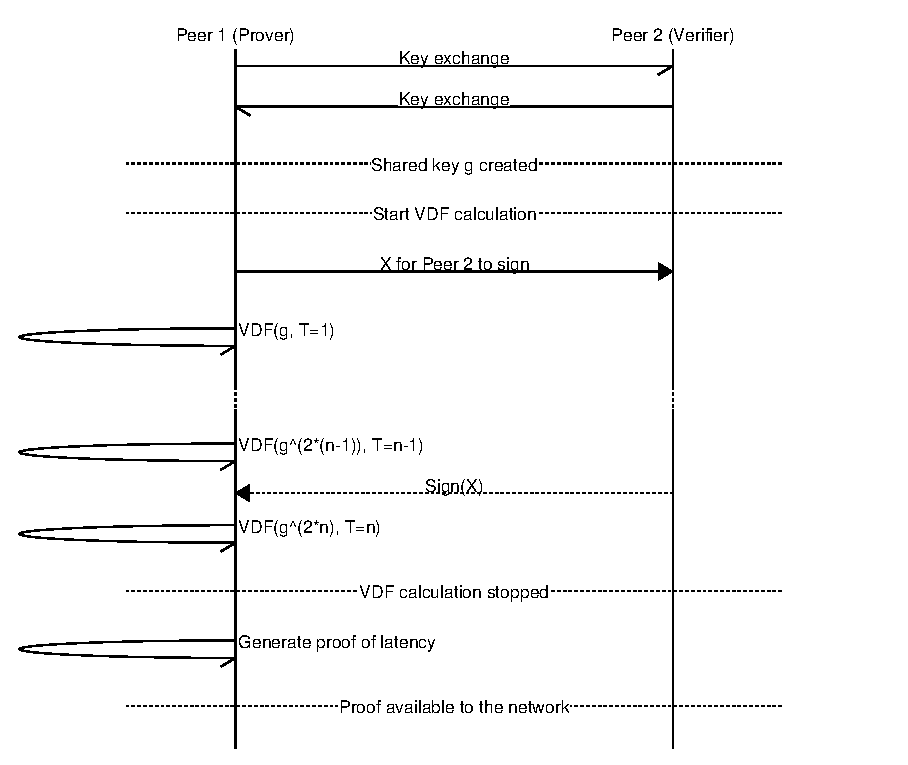
\includegraphics[width=\textwidth]{pictures/pol_diagram.eps}
\caption{Protocol diagram of Proof of Latency}
\label{Diagram 1}
\end{figure}
